\documentclass[tt2]{penoverslag}

%%% PACKAGES
\usepackage{lipsum}
\usepackage{gensymb}
\usepackage [dutch] {babel}
\usepackage{graphicx}
\usepackage{amsmath}
\usepackage{listings}
\usepackage{subcaption}
\usepackage{lscape}
\usepackage[absolute]{textpos}
  \setlength{\TPHorizModule}{1cm}
  \setlength{\TPVertModule}{1cm}


\begin{document}

\team{Zilver} % teamkleur
\members{Sam Gielis\\
         Sophie Marien\\
         Toon Nolten\\
         Nele Rober\\
         Gerlinde Van Roey\\
         Maxim Van Mechelen} % teamleden

\maketitlepage

\newpage

\begin{abstract}
\label{ssec:abstract}
Het P\&O-project heeft als doel vier autonome robots \textit{Team Treasure Trek} te laten spelen. Dit verslag beschrijft de invulling die team Zilver aan het project gaf.\\

De robot is voorzien van een lichtsensor, een infraroodsensor en een ultrasone sensor. Verder heeft de robot van een strip klittenband vooraan waarmee hij het voorwerp kan oprapen.
De robot kan een doolhof verkennen en hiervan een map bijhouden. Via RabbitMQ kunnen de robots en simulatoren met elkaar communiceren. Zo kunnen ze een map naar elkaar doorsturen om naar elkaar toe te rijden.\\

Een computerprogramma simuleert de werking van robots. Deze simulator kan vier robots tegelijk simuleren of kan in hybride vorm gebruikt worden (waarbij bijvoorbeeld \'e\'en fysieke en drie virtuele robots gebruikt worden). De gesimuleerde robots gedragen zich volledig analoog aan de fysieke robot.
\end{abstract}

\setcounter{tocdepth}{2}
\tableofcontents
%figuur robot
\begin{figure}[!hb]
\begin{textblock}{38}(4,15)
    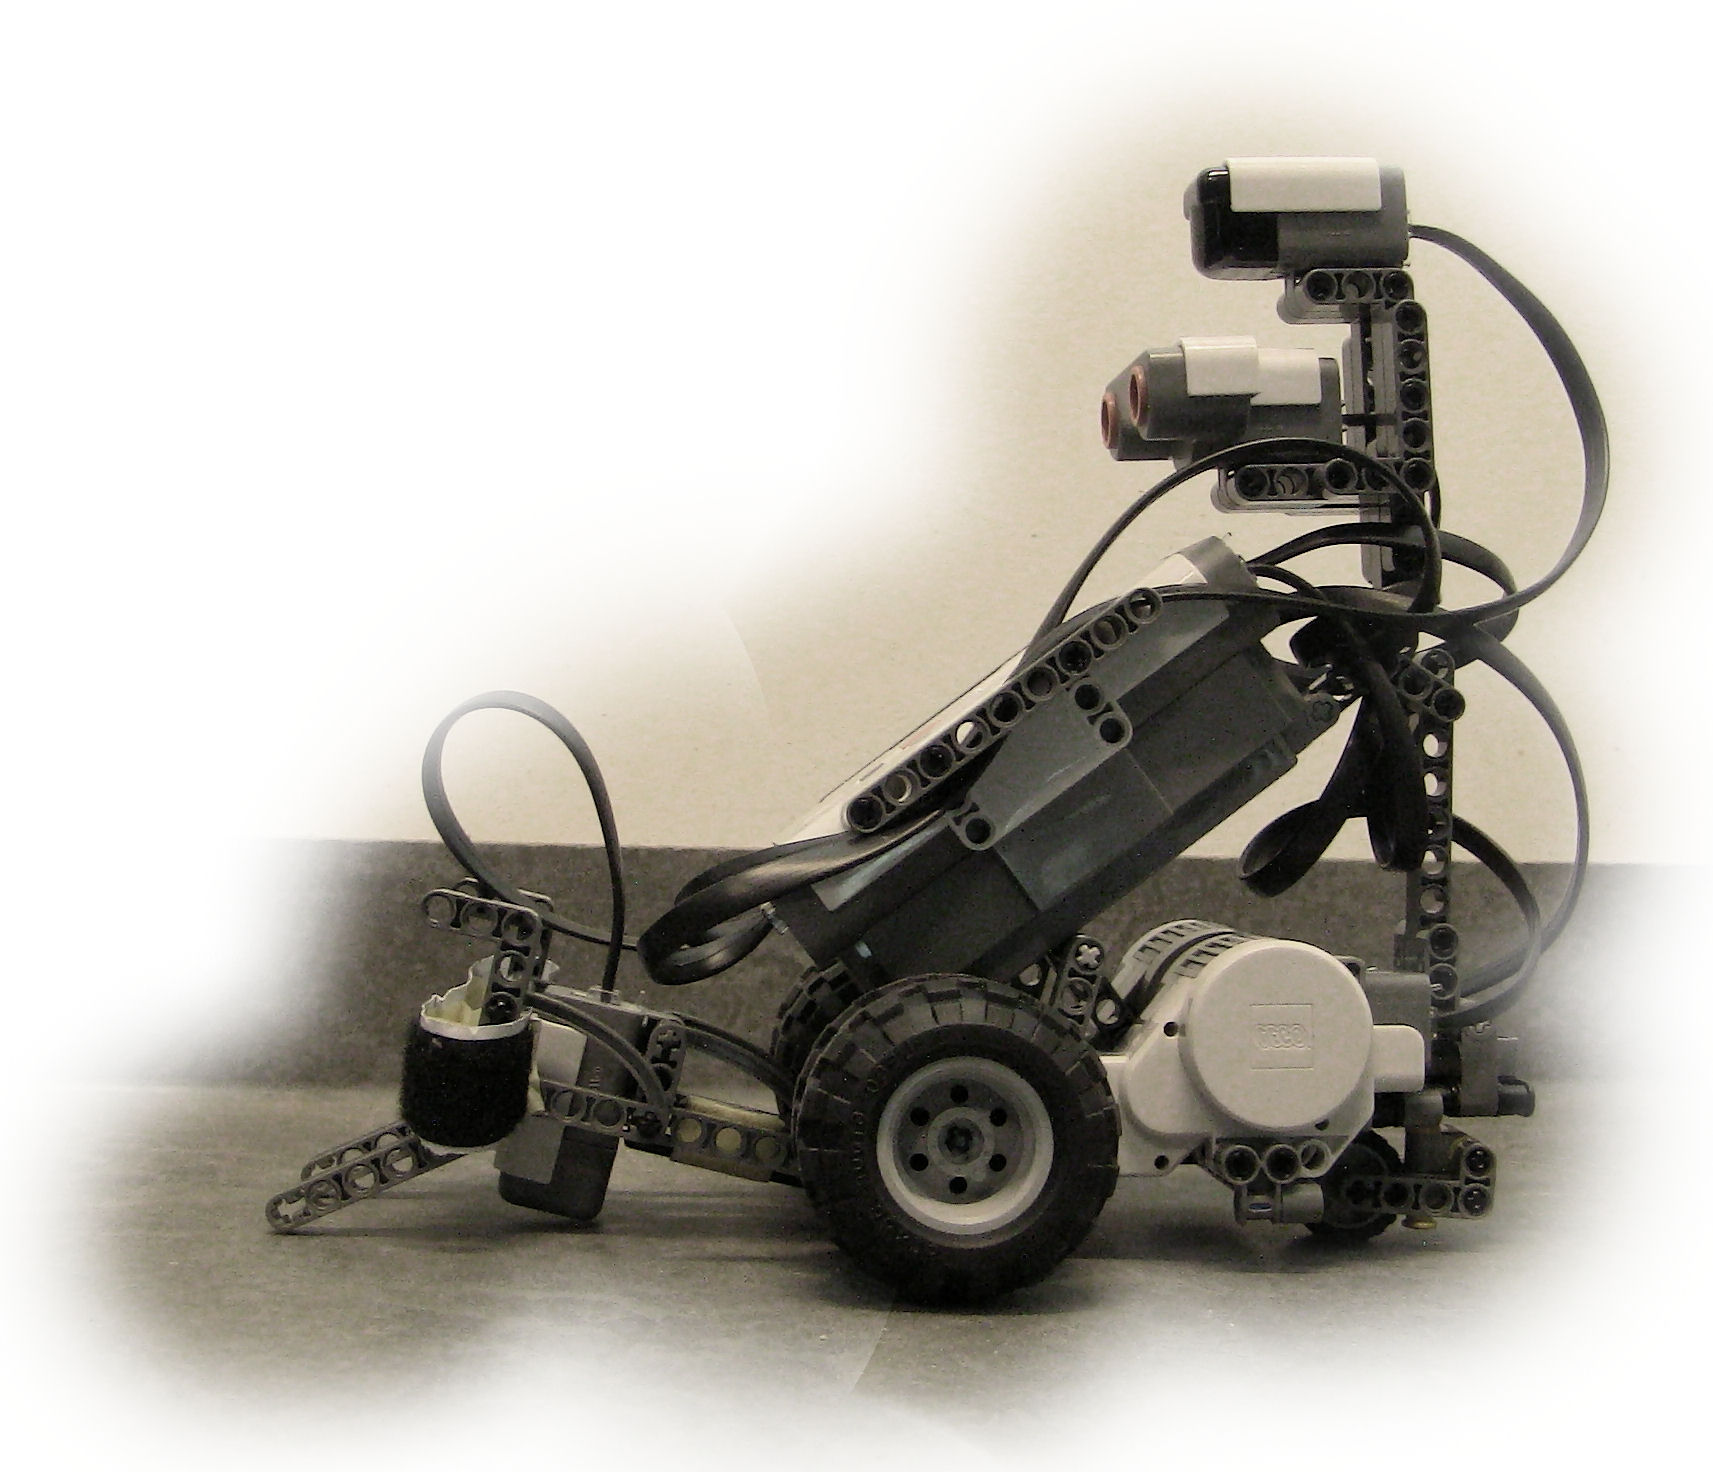
\includegraphics[width=0.45\textwidth]{robotFP}
    \label{fig:robotFP2}
\end{textblock}
\end{figure}

\newpage


% == INLEIDING == %
\section{Inleiding} % 4 ok
\label{ssec:inl}
In het kader van het vak `Probleemoplossen en Ontwerpen: computerwetenschappen' wordt gewerkt rond autonome intelligente robots. Verschillende teams bouwen en programmeren een robot met behulp van LEGO Mindstorms. Deze robot moet uiteindelijk samen met drie andere robots volledig autonoom \textit{Team Treasure Trek} kunnen spelen.
De robots moeten hierbij in een onbekend doolhof op zoek naar een bepaald voorwerp (een wc-rol). Elke robot krijgt een eigen voorwerp toegewezen. Wanneer een robot zijn voorwerp gevonden heeft, komt hij te weten met welke robot hij moet samenwerken. Elk duo moet beide voorwerpen bij elkaar brengen. Het duo dat hier eerst in slaagt, wint.\\

Voor de tweede demonstratie wordt met \'e\'en fysieke en drie gesimuleerde robots gewerkt. Het is ook mogelijk met vier virtuele robots te werken. De doolhof bevat mogelijk een wip. De robots zijn in staat hun eigen voorwerp te vinden en op te rapen. Wanneer een robot weet wie zijn teamgenoot is, kan hij hiermee een punt afspreken om samen te komen.\\


\section{Bouw robot}
\label{ssec:bouwrob}
LEGO Mindstorms biedt een bouwpakket voor een robot aan. Een NXT-microcomputer laat toe de robot te programmeren. Met behulp van leJOS kan dit in Java.

\subsection{Fysieke bouw}
\label{ssec:fysb}
Een infraroodsensor werd gemonteerd bovenop de robot. Door een infraroodbal onder een wip te plaatsen, kan de robot bepalen of de wip naar beneden staat. In dat geval wordt het infrarood licht immers geblokt. Later kan de infraroodsensor eventueel gebruikt worden om robots te detecteren.\\

Het voorwerp kan op verschillende manieren worden opgeraapt. Enkele opties werden getest: een schep met motor achteraan, een kartonnen schep vooraan en een plastieken schep met klittenband vooraan. Figuur \ref{fig:robotBouw} geeft deze opstellingen weer. Het testen van de opstellingen, leidde tot volgende bevindingen:

\begin{enumerate}
\item De robot heft het voorwerp expliciet op met behulp van een extra motor. Deze opstelling maakt de robot te lang waardoor hij moeilijk kon draaien zonder tegen een muur te botsen. Er werd besloten de schep vooraan te plaatsen.
\item Vooraan is niet genoeg plaats voor een extra motor, deze kon dus niet meer gebruikt worden. Een halve wc-rol leek een ideale vorm voor de schep. Na testen bleek dit echter niet altijd te werken.
\item De robot neemt het voorwerp op met behulp van klittenband. De schep zorgt ervoor dat het voorwerp niet over de grond sleept. Dit is de huidige opstelling.
\end{enumerate}

De infrarood- en ultrasone sensor staan vast gemonteerd op de robot. De schep werd samen met de lichtsensor scharnierend gemonteerd. Wanneer het hefboomsysteem de wip raakt, kantelt het omhoog. Zo kan de robot vlot de wip op.

De robot is ook voorzien van een dubbel paar wielen. Dit vermijdt dat hij van de wip glijdt.

Figuur \ref{fig:robotDetail} geeft details van de schep, de wielen en de sensoren.

% bouw robot
\begin{figure}
\centering
	\begin{subfigure}[h]{0.325\textwidth}
	\centering
		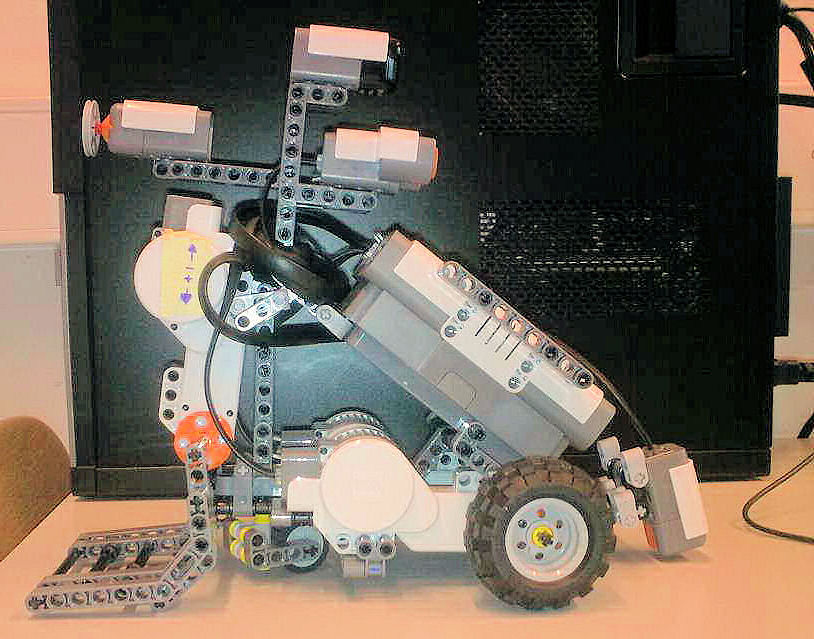
\includegraphics[width=\textwidth]{robotOud1}
		\caption{opstelling 1}
	\end{subfigure}
	\begin{subfigure}[h]{0.325\textwidth}
		\centering
		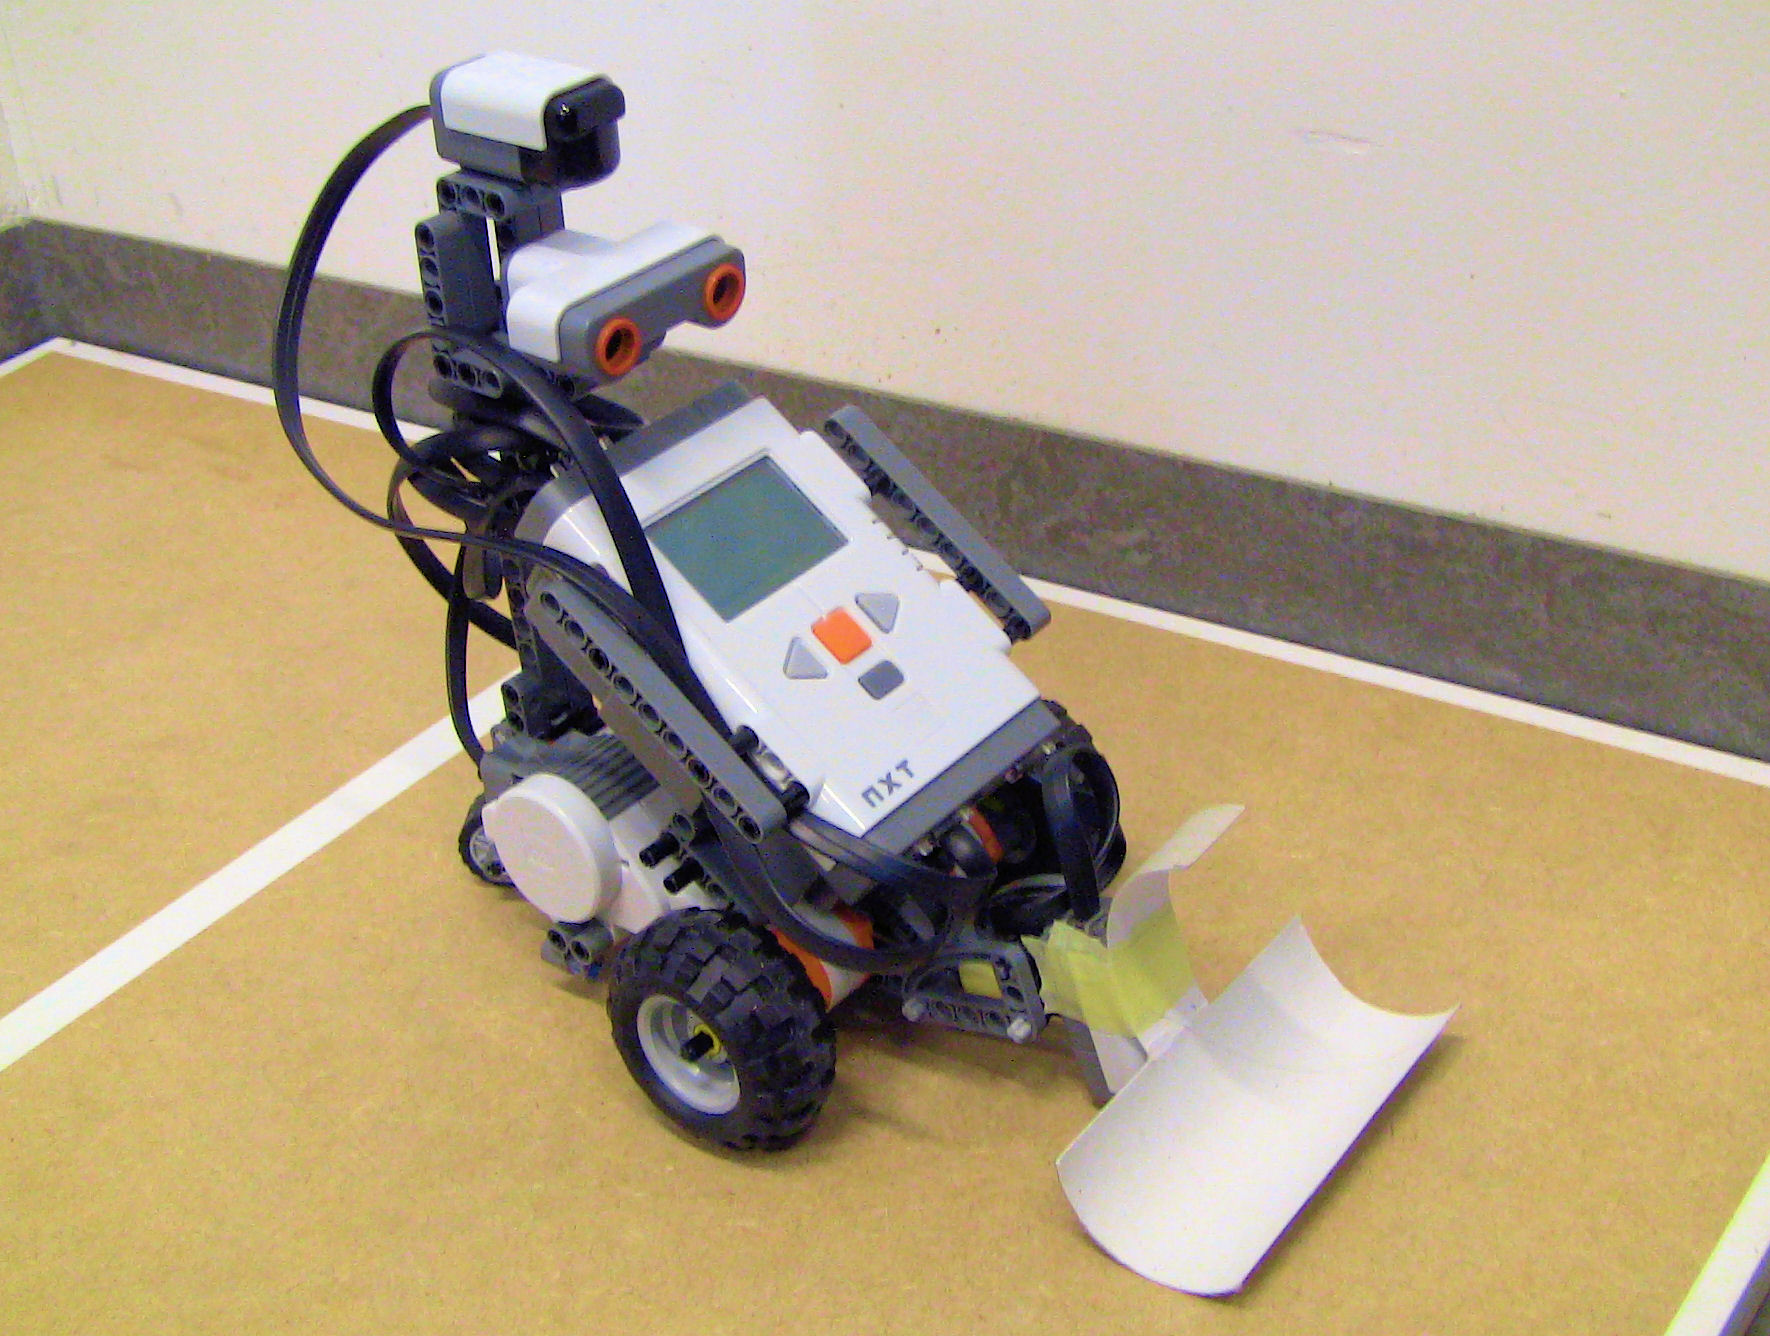
\includegraphics[width=\textwidth]{robotOud2}
	\caption{opstelling 2}
	\end{subfigure}
	\begin{subfigure}[h]{0.325\textwidth}
		\centering
		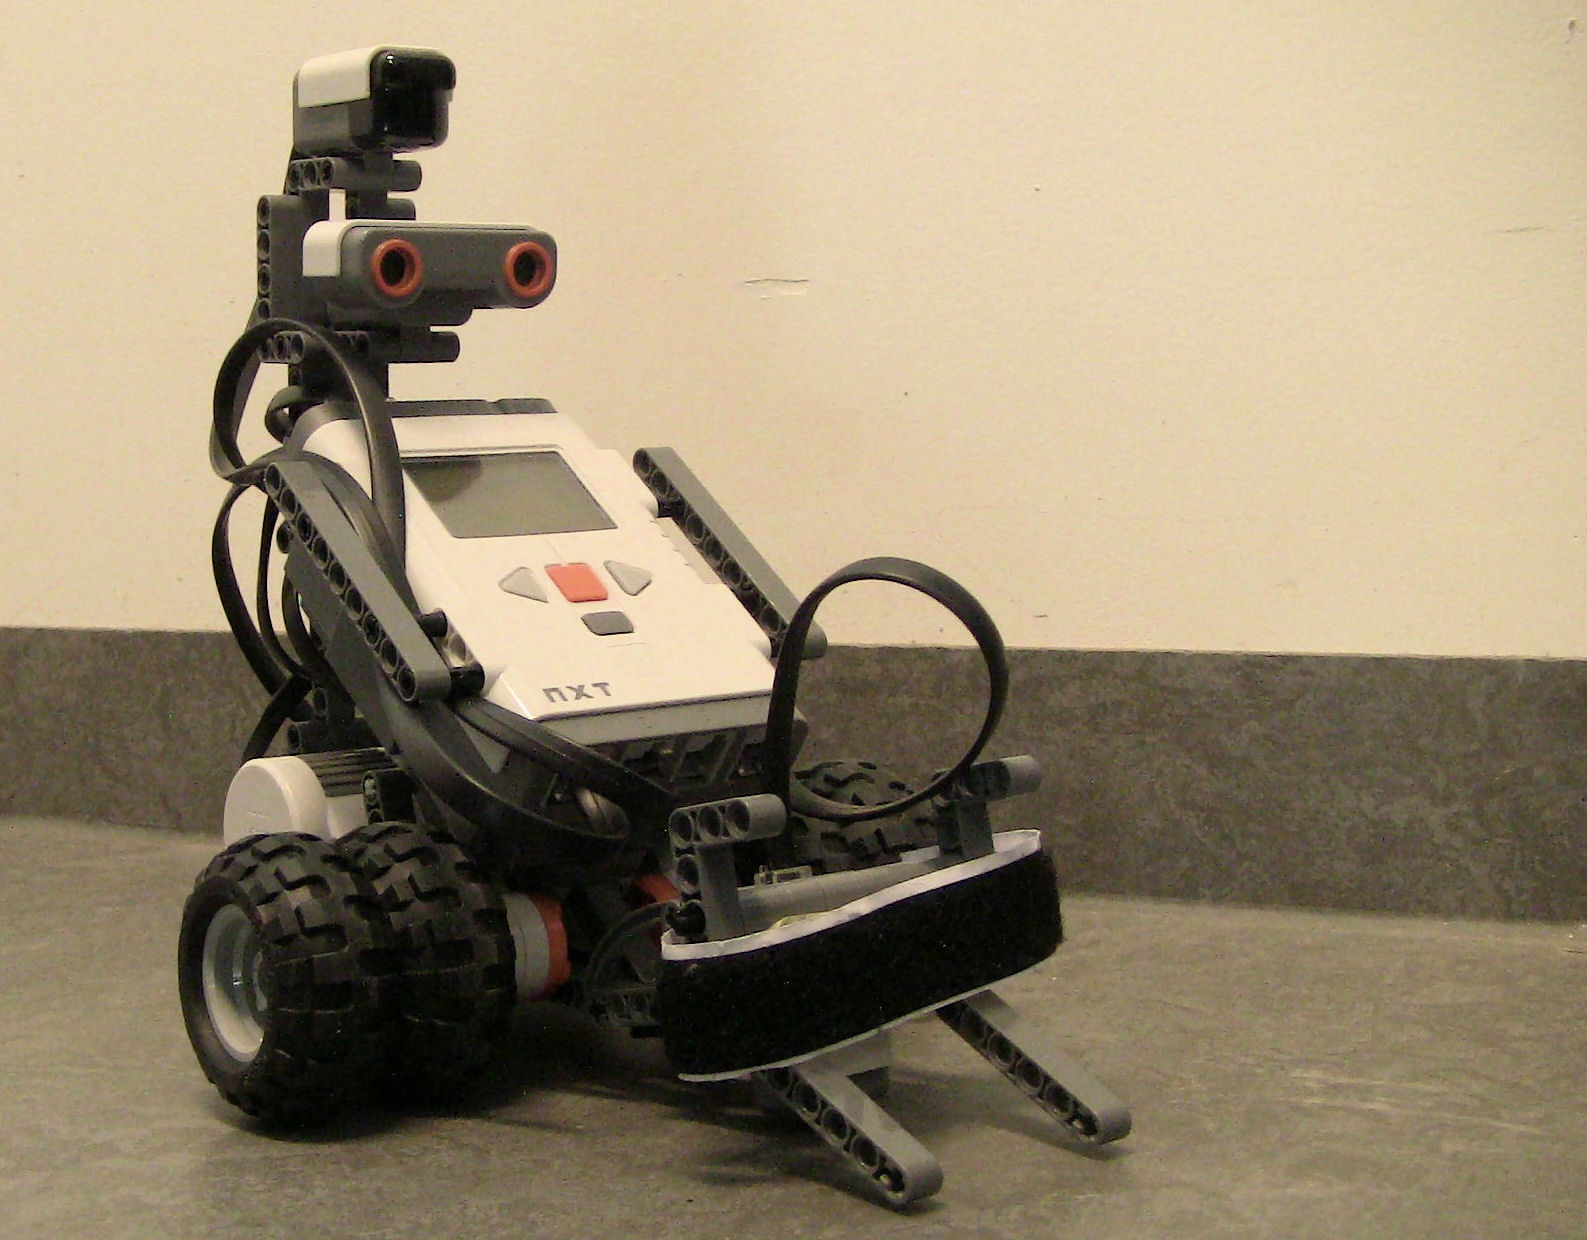
\includegraphics[width=\textwidth]{robotNieuw}
	\caption{opstelling 3}
	\end{subfigure}
\caption{Een vergelijking tussen verschillende ontwerpen.}
\label{fig:robotBouw}
\end{figure}

% details robot
\begin{figure}
\centering
	\begin{subfigure}[h]{0.325\textwidth}
	\centering
		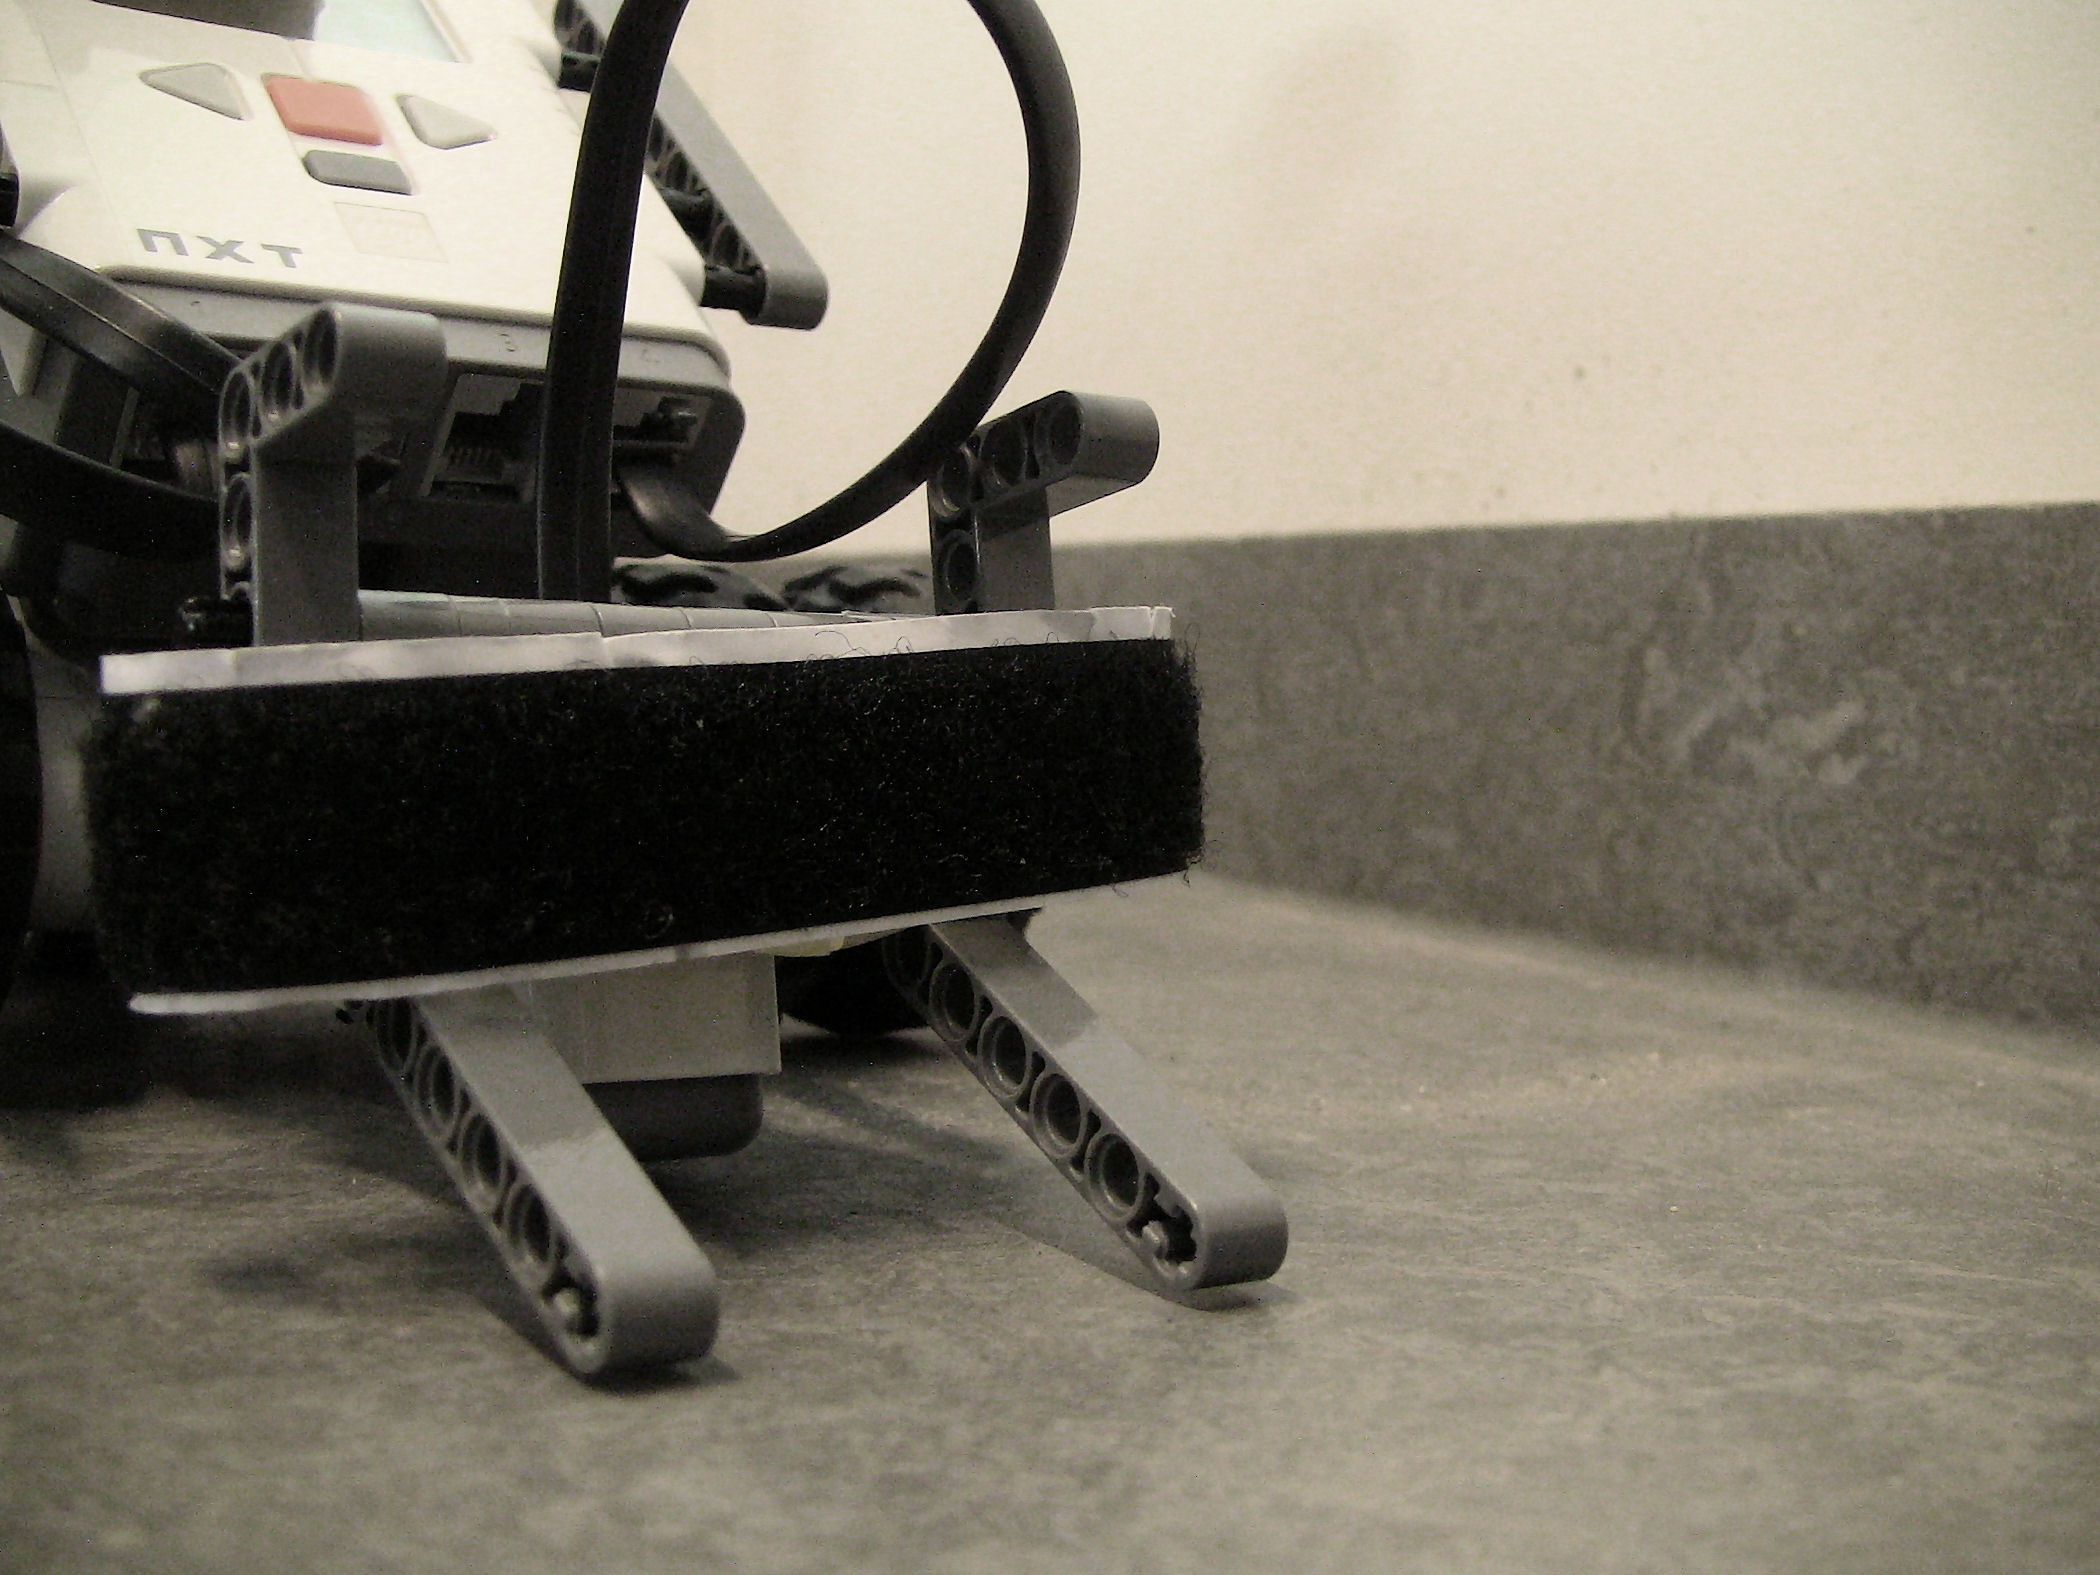
\includegraphics[width=\textwidth]{robotSchep}
		\caption{schep}
	\end{subfigure}
	\begin{subfigure}[h]{0.325\textwidth}
		\centering
		\includegraphics[width=\textwidth]{robotWielen}
		\caption{wielen}
	\end{subfigure}
	\begin{subfigure}[h]{0.325\textwidth}
		\centering
		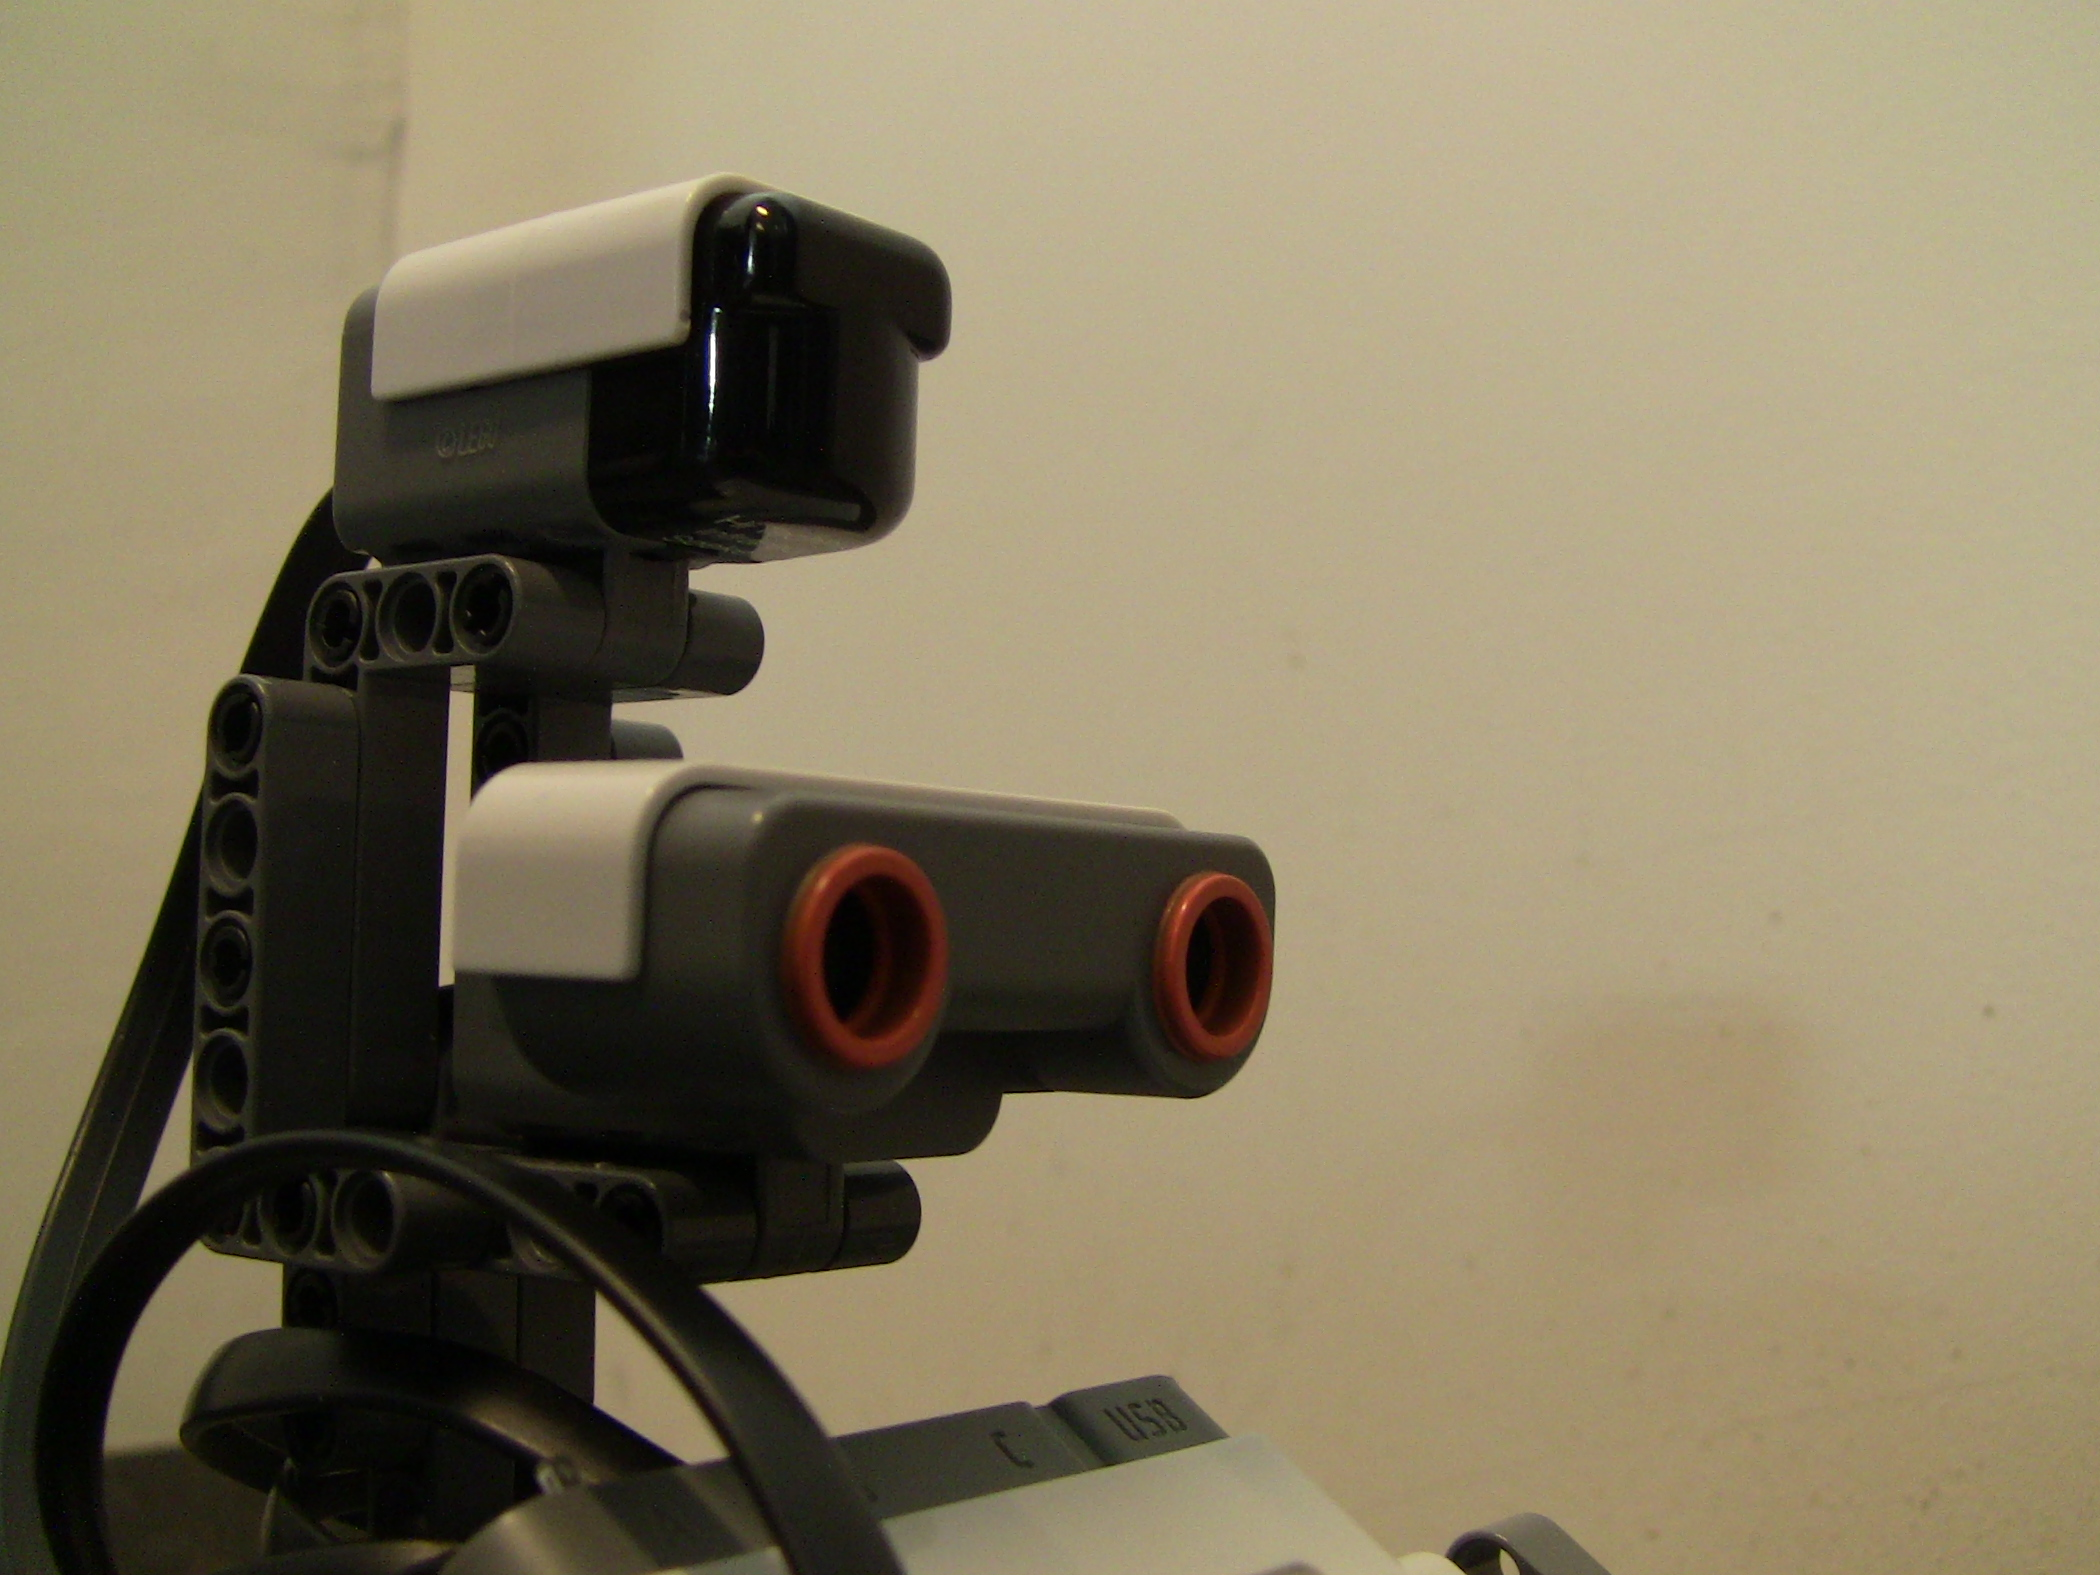
\includegraphics[width=\textwidth]{robotSensoren}
		\caption{infrarood- en ultrasone sensor}
	\end{subfigure}
\caption{Details van de robot.}
\label{fig:robotDetail}
\end{figure}


% == ALGORITMES == %
\section{Algoritmes}
Voor volgende algoritmes wordt verwezen naar het verslag van het eerste semester. Deze algoritmes worden dit semester zonder aanpassingen opnieuw gebruikt:
\begin{itemize}
	\item Rechtzetten op een witte lijn
	\item Centreren aan de hand van twee muren
	\item Lezen van een barcode
	\item Vinden van het kortste pad
\end{itemize}

% == zoeken van het voorwerp == %
\subsection{Zoeken van het voorwerp} %
\label{ssec:algoZoek}
Om het voorwerp te vinden moet de robot aanvankelijk het doolhof verkennen. In de loop van het eerste semester werd hiervoor een algoritme ontwikkeld. Dit werd verder geoptimaliseerd: 

\begin{description}
\item[A] basisalgoritme zonder optimalisatie: draai bij elke tegel vier keer (eindig in startori\"entatie) en neem de laatste tegel in de queue als volgende tegel.
\item[B] neem steeds de buur die met het minst aantal rotaties bereikt kan worden als volgende tegel.
\item[C] draai bij elke tegel slechts drie keer (eindig niet meer in startori"entatie).
\item[D] muren die vanuit een naburige tegel reeds gedetecteerd werden, worden niet nog eens nagekeken.
\item[E] tegels waarvan de vier zijden al gekend zijn en waaraan drie muren grenzen, worden niet meer bezocht (`dead-ends' kunnen onmogelijk barcodes bevatten, dus dit is geen probleem)
\end{description}

Bij de start van het tweede semester werd besloten een extra optimalisatie (F) toe te voegen. Deze geeft prioriteit aan tegels met voorwerpen. Een voorwerp kan zich enkel bevinden op een `dead-end', voorafgegaan door een `straight' met een barcode. De barcode identificeert het voorwerp. Wanneer de robot een mogelijke voorwerplocatie vindt, controleert hij zo snel mogelijk of er werkelijk een voorwerp ligt en om welk voorwerp het gaat. \\

\begin{figure}[!hb]
\centering
	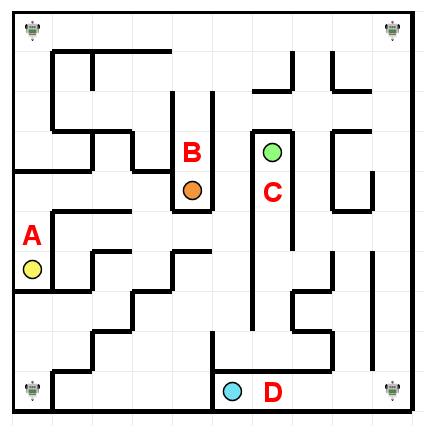
\includegraphics[scale=0.5]{doolhof3}
	\caption{Een doolhof waarop optimalisatie F van het verkenalgoritme getest werd.}
\label{doolhof3}
\end{figure}

\begin{table}[!hb]
\begin{center}
    \begin{tabular}{ c | c || c | c }
    \multicolumn{4}{c}{\textbf{Start linksboven}} \\ 
   \multicolumn{2}{c||}{Met dead-end prioriteit} & \multicolumn{2}{|c}{Zonder dead-end prioriteit}\\
     gevonden locatie & afgelegde weg (cm) & gevonden locatie &  afgelegde weg (cm)\\ \hline\hline
    A & {\color{green}720} & B & {\color{green}880} \\ \hline
    B & {\color{green}1520} & D & {\color{green}2960} \\ \hline
    D & {\color{green}4320} & C & {\color{green}4520} \\ \hline
    C & {\color{red}6120} & A & {\color{red}5920}\\
    \end{tabular}
    \caption{Testresultaten optimalisatie F, start linksboven}
    \label{tab:resultVerken}
\end{center}
\end{table}

\begin{table}[!hb]
\begin{center}
    \begin{tabular}{c | c || c | c }
    \multicolumn{4}{c}{\textbf{Start rechtsonder}} \\
   \multicolumn{2}{c||}{Met dead-end prioriteit} & \multicolumn{2}{|c}{Zonder dead-end prioriteit}\\
     gevonden locatie &  afgelegde weg (cm) & gevonden locatie &  afgelegde weg (cm)\\ \hline\hline
    D & 120 & D & 120 \\ \hline
    A & {\color{red}2920} & A & {\color{red}2600} \\ \hline
    B & {\color{red}3720} & B & {\color{red}3240} \\ \hline
    C & {\color{red}6240} & C & {\color{red}6000}\\
    \end{tabular}
    \caption{Testresultaten optimalisatie F, start rechtsonder}
    \label{tab:resultVerken}
\end{center}
\end{table}

Testresultaten: De figuur~\ref{doolhof3} geeft het geteste doolhof weer. Hierbij hebben we de robot acht keer laten rijden op vier verschillende posities. De tabellen geven de resultaten van de robot die start op de tegel met co"ordinaat 09 (dat is de rechterbovenhoek) en van de robot die start op de tegel met co"ordinaat 99 (dat is rechterbenedenhoek). De twee andere tabellen van de andere posities zijn niet weergegeven, maar die testresultaten zijn er wel. De robot heeft twee maal het doolhof verkend. De eerste keer met de dead-end prioriteit en de tweede keer zonder dead-end prioriteit. Als de kleuren groen zijn in de tabel betekent dat het met dead-end prioriteit beter was, en als de kleur rood is van de getallen dan is het niet voordelig om dead-end prioriteit te gebruiken. Uiteindelijk zijn deze testen uitgevoerd op 4 verschillende hoeken beginnend uit elke hoek, maar deze testresultaten waren teveel om in het verslag bij te voegen.\\


Uit deze testen blijkt dat het algoritme vaker effici"enter is zonder deze optimalisatie. Dit komt omdat de robot veel omrijdt om het dichtstbijzijnde vakje te vinden en daardoor meermaals hetzelfde pad op en afgaat. Het is immers moeilijk het kortste pad naar de voorwerplocatie te bepalen omdat deze tegels vaak nog niet verkend zijn. Uit deze resultaten hebben we besloten om de optimalisatie niet door te voeren maar het oorspronkelijke algoritme te behouden. \\

Nadat het voorwerp gevonden is, probeert de robot zijn teamgenoot te contacteren. Indien de teamgenoot zijn voorwerp nog niet heeft of wanneer de mappen van beide robots nog niet combineerbaar zijn, gaat de robot verder met het verkennen van het doolhof. \\

\subsection{Weg vinden naar andere robot}
Hierbij dachten we aan het kortste-pad-algoritme. Dit zal wel nog aangepast moeten worden aan zowel draaien als vooruit rijden (draaien was nog niet in rekening gebracht).\\ Er moet ook nog rekening gehouden worden als de andere robot zou wegrijden. De robot mag hierdoor niet in een loop terechtkomen. \\

In de scheidsrechterscommissie is er besloten dat de robots naar elkaar informatie doorsturen over waar ze zich bevinden in het doolhof. Dit kan gebeuren via de hele verkende map door te sturen. De robot kan er dan voor kiezen om delen van de informatie van zijn teamgenoot te gebruiken of niet. Met deze informatie rijdt de robot naar zijn teamgenoot. Ze spreken geen tegel onderling af, maar rijden gewoon naar elkaar toe. Dit heeft het nadeel dat als ze elk een ander pad kiezen ze elkaar kunnen kruisen zonder dat ze het weten. Voorlopig wordt dit dus toegepast in deze demo.\\

% == SOFTWARE == %
\section{Software}
\label{secc:softw}
De software bestaat uit twee delen: een project dat op de NXT van de robot loopt en een project dat op de computer loopt (sectie \ref{ssec:Sdesign}). Alles wordt aangestuurd via de \textit{Graphical User Interface (GUI)} (sectie \ref{ssec:GUI}). Deze laat toe de robot te besturen en de reacties van de robot weer te geven. Robots kunnen met elkaar communiceren via RabbitMQ (sectie \ref{ssec:RabbMQ}). Via de GUI kunnen ook virtuele robots aangestuurd worden: de simulators (sectie \ref{ssec:Sim}).\\

Voor volgende secties wordt verwezen naar het verslag van het eerste semester. Deze implementaties en ontwerpen werden zonder aanpassingen opnieuw gebruikt:

\begin{itemize}
\item Commando's doorgeven
\item Bluetooth
\item Robot
\end{itemize}

% -- Ontwerp -- %
\subsection{Ontwerp van het computerproject}
\label{ssec:Sdesign}
Een overzicht van het ontwerp wordt weergegeven in de klassendiagramma van figuur \ref{fig:klasSoft}.\\

% klassendiagram
\begin{figure}
\centering
		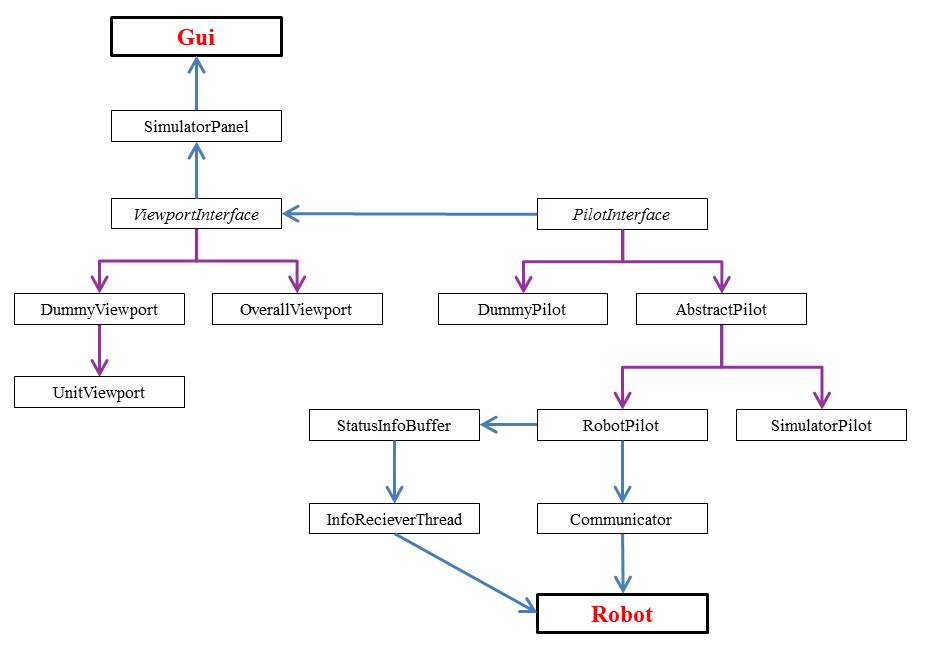
\includegraphics[width=\textwidth]{KlasSoftware}
\caption[Klassendiagram computerproject]{Klassendiagram met de belangrijkste klassen van het computerproject (paarse pijlen wijzen op overerving of implementatie, blauwe op een informatiestroom)}
\label{fig:klasSoft}
\end{figure}

De Main-methode bevindt zich in de GUI-klasse. Deze maakt een \textit{SimulatorPanel}-object aan. Dit is een overkoepelend panel waarin meerdere \textit{Viewports} zitten. Een \textit{OverallViewport} geeft het volledige doolhof en alle robots erin weer. Dit kan uiteraard enkel wanneer een gekend virtueel doolhof gebruikt wordt en wanneer van alle robots genoeg informatie beschikbaar is. Een \textit{UnitViewport} geeft de wereld van \'e\'en robot (eventueel gesimuleerd) weer: de sensorwaarden en de muren die hij reeds ontdekt heeft. Een wereld waarvan niets geweten is, kan niet worden weergegeven. Dit is het geval voor robots van andere teams: zij worden niet weergegeven in de GUI, met uitzondering van de teamgenoot. Deze laatste stuurt wel zijn map door, maar niet zijn sensorwaarden en wordt gerepresenteerd door een \textit{DummyViewPort}. Het aantal \textit{Viewports} hangt af van het aantal gekende werelden.\\

Een \textit{DummyViewport} is aanvankelijk leeg. Wie de teamgenoot van de robot is, wordt immers pas bekend wanneer beide leden van het team hun voorwerp gevonden hebben. Op dat moment zal de \textit{DummyViewport} iets weergeven.\\

Elke \textit{Viewport} krijgt een eigen \textit{Pilot} toegewezen (behalve \textit{OverallViewport}, die krijgt er meerdere). Er zijn verschillende soorten \textit{Pilots} die elk een implementatie van \textit{PilotInterface} zijn. De keuze van \textit{Pilot} hangt af van het type robot. Een robot waarvan de wereld niet kan worden voorgesteld, krijgt geen \textit{Pilot}. Een teamgenoot (die we niet zelf simuleren) heeft een \textit{DummyPilot}. Deze bevat enkel `getters', want deze robot kan niet worden aangestuurd. Een robot die gesimuleerd wordt, heeft een \textit{SimulatorPilot}. Deze berekent zelf zijn sensorwaarden op basis van een virtuele doolhof. Een fysieke robot krijgt een \textit{RobotPilot} die via de \textit{Communicator} in verbinding staat met de fysieke robot. De \textit{RobotPilot} krijgt zijn sensorwaarden terug van de robot via de \textit{InfoReceiverThread} en de \textit{StatusInfoBuffer}. Deze \textit{Pilots} zijn de `hersenen' van deze robots/simulators. De \textit{Viewports} geven enkel weer wat de robots uitvoeren, zij berekenen en beslissen niets.

% -- GUI -- %
\subsection{Grafische User Interface}
\label{ssec:GUI}

% figuur GUI
\begin{figure}[h]
\centering
	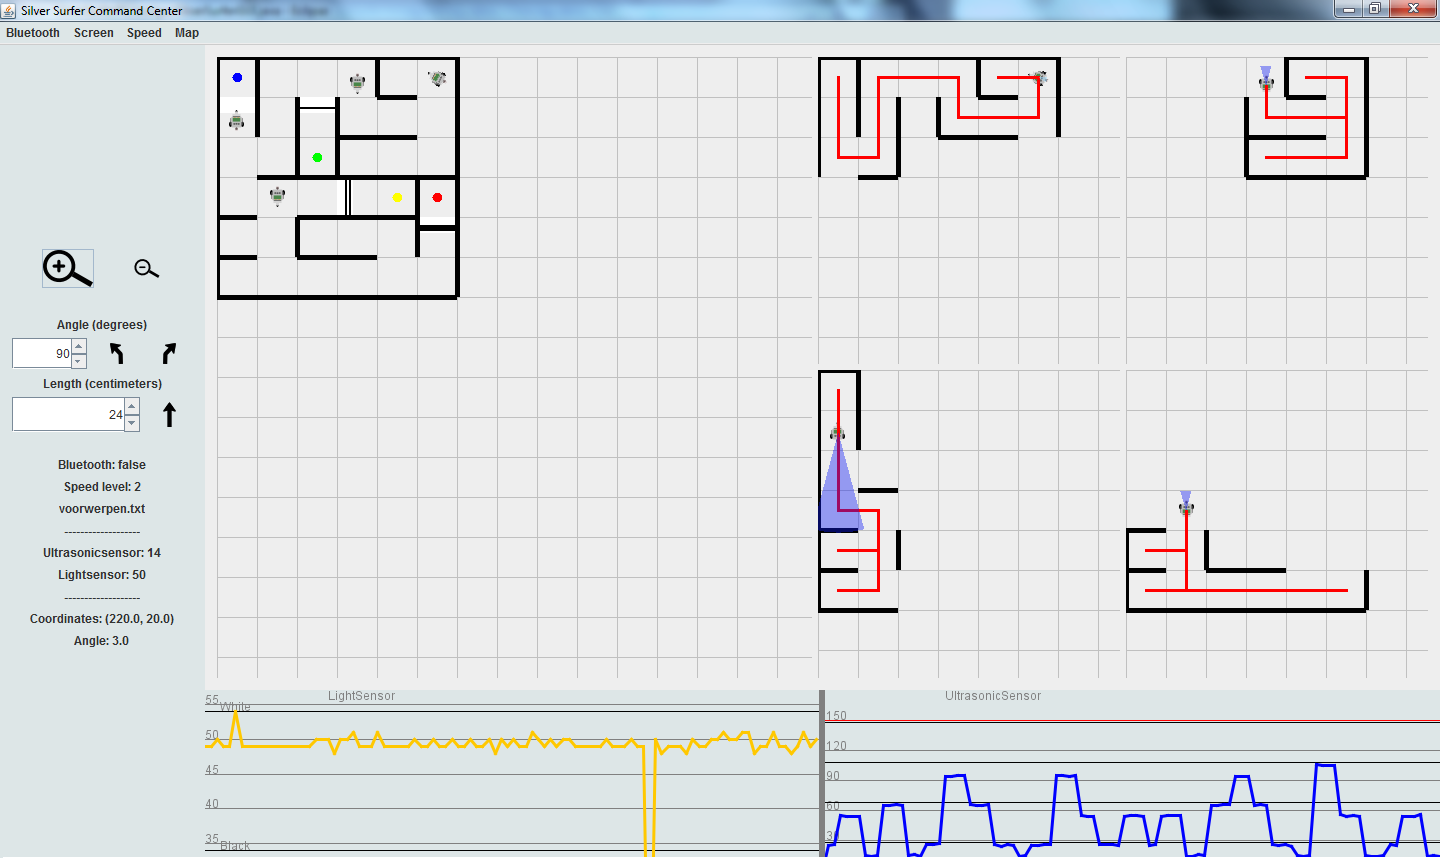
\includegraphics[width=0.8\textwidth]{GUInew}
\caption{de Graphical User Interface}
\label{fig:GUI}
\end{figure}

De GUI van deze demo werkt voorlopig niet dus is hier geen foto van beschikbaar. De figuur van de GUI zoals deze er in de vorige demo uit zag, wordt weergegeven in figuur \ref{fig:GUI}.\\

Het eerste doolhof is de overal \textit{Vieuwport} met de vier verschillende robotten.  De objecten worden voorgesteld door gekleurde bollen. Elke robot heeft initieel een eigen kleur, weergegeven als een gekleurde cirkel onder de robot. Zo is gemakkelijk te zien welk object bij welke robot hoort. Wanneer een robot zijn object gevonden heeft, zal zijn kleur veranderen in de teamkleur. Wanneer alle robots hun object gevonden hebben, zullen er dus twee teams van twee robots zijn, elk met dezelfde kleur.

%De GUI zal er wat anders uitzien dan vorig semester. Het moet nu immers mogelijk zijn de wereld van meerdere robots tegelijk weer te geven. Deze werelden verschillen van elkaar: zeker in het begin verkennen de verschillende robots een ander deel van het doolhof. Omdat zowel beginpositie als -ori\"entatie niet gekend zijn, is het niet mogelijk al deze werelden in \'e\'en paneel weer te geven. Het \textit{SimulatorPanel} wordt opgedeeld in verschillende \textit{Viewports}. Zoals uitgelegd in sectie \ref{ssec:Sdesign} hangt het aantal \textit{Viewports} af van de situatie.\\

%Objecten worden voorgesteld door gekleurde bollen. Elke robot heeft initieel een eigen kleur, weergegeven als een gekleurde cirkel onder de robot. Zo is gemakkelijk te zien welk object bij welke robot hoort. Wanneer een robot zijn object gevonden heeft, zal zijn kleur veranderen in de teamkleur. Wanneer alle robots hun object gevonden hebben, zullen er dus twee teams van twee robots zijn, elk met dezelfde kleur.

Wanneer de robot een pad aflegt, tekent de \textit{UnitViewport} dit in het tekenpaneel als een rode lijn (herschaald: \'e\'en cm = \'e\'en pixel). De lijnen worden als lijnen opgeslagen in de \textit{UnitViewport}. Wanneer de robot een rechte weg aflegt, wordt het eindpunt van de gedefinieerde lijn steeds verlegd. Dit zorgt ervoor dat de weg die de robot aflegt continu bijgewerkt wordt. De huidige positie en de huidige ori\"entatie van de robot worden weergegeven door een driehoek die draait met de ori\"entatie. Het bereik van de ultrasone sensor wordt grafisch weergegeven met een blauwe boog. De lichtsensor wordt voorgesteld als een bol die van kleur verandert wanneer de ondergrond wijzigt. 
Een \textit{DummyViewport} geeft geen pad of sensorwaarden weer, enkel een map. De map-in-opbouw wordt weergegeven op basis van de map die de \textit{Pilot} opstelt.\\

Al deze \textit{Viewports} nemen plaats in, waardoor andere functionaliteiten van de GUI naar de achtergrond moeten verdwijnen. De sensorgrafieken, bijvoorbeeld, zullen nog beschikbaar zijn, maar worden enkel zichtbaar wanneer deze via een menu expliciet geopend worden. Zo kunnen ze nog steeds gebruikt worden voor testen.



% -- RabbitMQ -- %
\subsection{Communicatie via RabbitMQ}
\label{ssec:RabbMQ}
De scheidsrechterscommissie ontwikkelde \textit{Het Team Treasure Trek Protocol (HTTTP)} en een implementatie ervan. De implementatie bevat o.a. een \textit{Client}-klasse die het gebruik van RabbitMQ bijna volledig abstraheert. Ook een \textit{Handler}-interface is voorzien. Deze moet door de teams zelf ge\"implementeerd worden.\\

Het computerproject bevat een \textit{PlayerHandler} en een \textit{SpectatorHandler}, om respectievelijk in de \textit{AbstractPilot} en de \textit{DummyPilot} met informatie om te gaan. Een onderscheid is nodig omdat \textit{DummyPilots} `aangestuurd' worden via hun handler. Figuur \ref{fig:KlasHTTTP} geeft een overzicht van de softwarearchitectuur.

Bij het aanmaken van een \textit{Pilot} wordt een \textit{MQCenter} aangemaakt met bijhorende \textit{Handler}. Het \textit{MQCenter} abstraheert de \textit{Client}-klasse nog verder.

% klassendiagram HTTTP
\begin{figure}[h]
\centering
	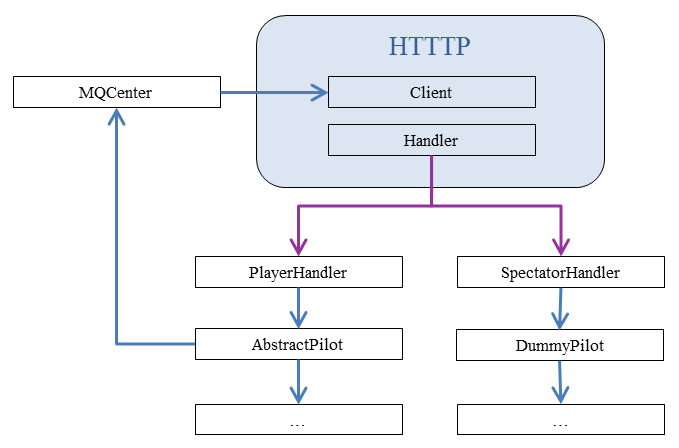
\includegraphics[width=0.8\textwidth]{KlasHTTTP}
\caption{Klassendiagram HTTTP}
\label{fig:KlasHTTTP}
\end{figure}


% -- Simulator -- %
\subsection{Simulator}
\label{ssec:Sim}
De \textit{Simulator} bootst de werking van de robot virtueel na. Hij kan dezelfde commando's uitvoeren als de werkelijke robot en simuleert de sensorwaarden die een echte robot zou genereren wanneer deze zich in een soortgelijke situatie bevindt.\\

De \textit{SimulatorPilot} bepaalt de positie van de `robot' ten opzichte van het virtuele doolhof: hoe ver van de muur en op welke ondergrond. De klasse \textit{SimulationSensorData} houdt sensorwaarden bij van tests op de echte robot in verschillende situaties. De \textit{SimulatorPilot} haalt hier zijn referenties uit en probeert op basis van de meetwaarden een realistische sensorwaarde te genereren. De sensorwaarden worden niet nauwkeurig gegenereerd: er wordt ruis toegevoegd. De echte robot geeft immers ook geen exacte waarden.\\

De \textit{AbstractPilot} bepaalt hoe de gesimuleerde robot moet reageren in de gegeven situatie. De klasse bevat methodes als \textit{travel()} en \textit{rotate()}. Ook bouwt de \textit{AbstractPilot} een map op terwijl de robot zich voortbeweegt door het doolhof. De \textit{AbstractPilot} kan zowel de echte robot als een gesimuleerde robot aansturen. De \textit{AbstractPilots} zijn de hersenen van de robots.

% -- Mapping -- %
\subsection{Mappen van een doolhof} % 3 ok
\label{ssec:mapping}
Het \textit{Mapping}-pakket heeft klassen zoals \textit{Tile}, \textit{Edge}, \textit{Obstruction} en \textit{Barcode} die elementen uit de wereld van een robot voorstellen.  Een \textit{Tile} stemt overeen met \'e\'en tegel van de doolhof en heeft vier \textit{Edges}: \'e\'en voor elke zijde. Die \textit{Edges} houden de twee aanliggende tegels bij en eventueel een \textit{Obstruction}, bijvoorbeeld een muur. De klasse \textit{MapGraph} brengt al deze elementen samen. Ze houdt een begin tegel bij en een huidige tegel. Ze biedt functionaliteiten aan om van de huidige tegel naar de tegel Noord, Oost, Zuid of West ervan te reizen en de map dynamisch uit te breiden. Zo wordt impliciet een hele graaf bijgehouden. De klasse \textit{MapReader} kan uit een bepaalde textfile een MapGraph opstellen die overeenkomt met de doolhof die in het bestand gedefinieerd wordt.\\

De \textit{Simulator} heeft een \textit{MapGraph} die de virtuele doolhof voorstelt. Tijdens het verkennen wordt een nieuwe \textit{MapGraph} opgesteld in de klasse \textit{SimulationPanel}, die de muren ook tekent. Ook de robot maakt gebruik van het \textit{SimulationPanel} om de verkende map op te slaan.

% klassendiagram HTTTP
\begin{figure}[h]
\centering
	\includegraphics[width=0.8\textwidth]{klasMapping}
\caption{Klassendiagram mapping}
\label{fig:KlasMap}
\end{figure}


% == BESLUIT == %
\section{Besluit}
De bouw van de robot wordt uitgebreid met een infraroodsensor bovenaan en een schep vooraan. De schep laat toe een voorwerp op te rapen. Op de schep is klittenband aangebracht zodat het voorwerp stevig vastzit. De lichtsensor heeft een scharnier gekregen. Zo zit de lichtsensor niet in de weg wanneer de robot over een wip rijdt. \\

De GUI ziet er anders uit dan vorig semester. Zo kunnen nu ook de tegenstanders en de teamgenoot gesimuleerd worden. Al deze robots (al dan niet gesimuleerd) hebben een eigen idee van de wereld. Deze verschillende werelden worden weergegeven via \textit{Viewports}.\\

Verder werd de communicatie ge\"implementeerd zodat de robot een bericht kan sturen wanneer hij zijn voorwerp vindt. 
De robot communiceert met andere robots via RabbitMQ. Zo kan de robot afspraken maken met anderen en kan hij te weten komen wie zijn teamgenoot is.
 


\newpage
\makeappendix

%% == DEMO 1 == %
\section{Demo 1} % 3
\label{Asec:demo1}
De robot wordt voor de eerste demo voorzien van een schep die bestaat uit een halve wc-rol. De infraroodsensor is ge\"installeerd, maar wordt nog niet gebruikt. Wanneer de robot zijn voorwerp vindt, stuurt hij een bericht via RabbitMQ. De GUI is opgesplitst in verschillende \textit{Viewports} die elk een of meerdere \textit{Pilots} weergeeft.

% == resulaten == %
\subsection{Resultaten} % 3 ?
\label{Assec:result1}
Het algoritme waarmee de robot zijn voorwerp opraapte, maakte gebruik van de travel() methode. De \textit{ExploreMaze}-thread wist echter niet dat de robot van plek was verandert. In de waan dat de robot op een andere plek stond dan in werkelijkheid, gaf de thread verkeerde instructies waardoor de robot tegen een muur reed. \\
Het schepsysteem van de robot functioneerde niet. Tijdens de demo faalde de robot toen hij het object moest oprapen. 

% == conclusies == %
\subsection{Conclusies} % 3 ?
\label{Assec:conc1}
Het bovengenoemd probleem is voor de volgende demo opgelost. Wanneer de \textit{ExploreMaze}-thread onderbroken wordt, zorgt de onderbrekende methode steeds dat de robot op dezelfde plek staat als waar de \textit{ExploreMaze}-thread denkt dat de robot staat.\\
Het opraapsysteem voor de robot is ook aangepast. De schep is weggehaald en er is een klittenband aangebracht. De robot is nog steeds in staat om het voorwerp met een scharnierend systeem op te heffen, zodat de robot vlot over de wip heen kan.


% == aanpassingen == %
\subsection{Oplijsting aanpassingen verslag} % 3 ?
\label{Assec:aanp1}
Volgende secties werden aangepast ten opzichte van de eerste demonstratie:

% overzicht aangepaste secties
\begin{itemize}
\item \textit{\ref{ssec:abstract} Abstract:} aangepast.
\item \textit{\ref{ssec:fysb} Fysieke bouw:} de schep vooraan werd aangepast.
\item \textit{\ref{ssec:algoZoek} Zoeken van het voorwerp:} testen van de prioriteit.
\item \textit{\ref{ssec:infra} Infraroodsensor:} Nieuw stuk over infraroodsensor werd toegevoegd, samen met de testen.
\item \textit{\ref{ssec:GUI}} Grafic user interface: de figuur van de GUI is aangepast en de tekst.


%\item \textit{calibratie infrarood}: nieuwe gegevens.
\end{itemize}



%\begin{thebibliography}{9}
%
%\bibitem{TeamTreasure} 
%\textit{Team Treasure Trek}: Een onderdeel van Mario Party 4. \mbox{[www.nintendo-europe.com/]}
%
%\bibitem{RabbitMQ}
%\textit{RabbitMQ}: Een communicatiesysteem dat het Advanced Message Queing Protocol (AMQP) implementeert. Door een kanaal op te zetten met een RabbitMQ-server is het mogelijk een bericht te plaatsen dat anderen kunnen lezen. De server heeft enkele `exchanges' die de berichten verdelen over `queues'. Die `queues' worden aangemaakt door de `clients' en luisteren elk naar een bepaald onderwerp. De `exchange' pushed dus berichten met een bepaald onderwerp naar de juiste `queues'.
%\mbox{[http://en.wikipedia.org/wiki/RabbitMQ]}
%
%\bibitem{mindstorms}
%\textit{Lego Mindstorms}:  Een uitbreiding op de LEGO bouwstenen waarmee kleine, aanpasbare en programmeerbare robots gebouwd kunnen worden. Een centrale besturingsmodule (`the brick') kan geprogrammeerd worden met verschillende programmeertalen. In eerdere versies werd een RCX gebruikt voor de brick, nu wordt met NXT gewerkt. De brick kan enkele motoren aandrijven. Bovendien kunnen er verschillende sensoren, o.a. een ultrasone sensor en een lichtsensor, aangesloten worden.  \mbox{[www.lego.com]} \mbox{[http://en.wikipedia.org/wiki/Lego\textendash Mindstorms]}
%
%\bibitem{leJOS}
%\textit{leJOS}: Een kleine Java Virtuele Machine die toelaat de NXT-brick te programmeren. leJOS voorziet verschillende klassen die o.a. de motoren aansturen en een bluetoothverbinding opzetten.  \mbox{[http://lejos.sourceforge.net/]}
%
%
%
%\end{thebibliography}



\end{document}
